\section{Theoretical Analysis}
\label{sec:analysis}

In this section, the circuit shown in Figure~\ref{fig:circuit} is analysed
theoretically, in terms of its time and frequency responses.

\subsection{Operating Point for t$<$0}
\label{subsec:tb0}

In this section the circuit is analysed for t$<$0, according to the Figure~\ref{fig:NodeMethod}, using the Node Method. Since the voltage source has a constant value $v_s(t)=V_s, t<0$, and assuming the circuit is stabilized, one can conclude that the the voltage in the capacitor is constant, therefore, the current that passes through it is $i_c=\frac{dv_c}{dt}=0$, and the capacitor can be replaced by an open circuit.\par

\begin{figure}[H] \centering
  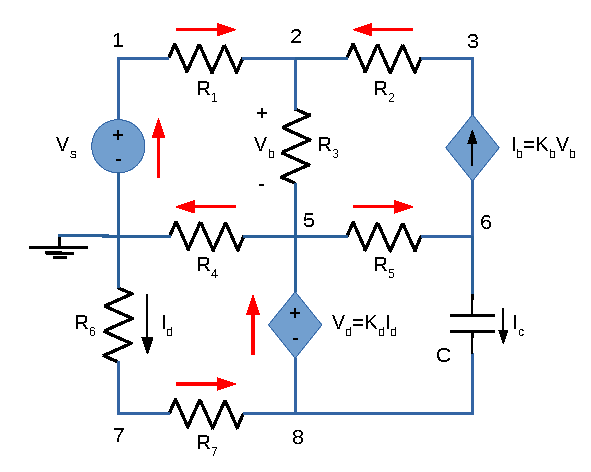
\includegraphics[width=0.7\linewidth]{NodeMethod.pdf}
  \caption{Currents Direction Identification}
  \label{fig:NodeMethod}
\end{figure}

The system solved is shown below:\par

$$
\begin{bmatrix}
  1 & 0 & 0 & 0 & 0 & 0 & 0 \\
  G_{1} & -G_{1}-G_{2}-G_{3} & G_{2} & G_{3} & 0 & 0 & 0 \\
  0 & G_{2}+K_{b} & -G_{2} & -K_{b} & 0 & 0 & 0 \\
  0 & G_{3} & 0 & -G_{3}-G_{4}-G_{5} & G_{5} & G_{7} & -G_{7} \\
  0 & -K_{b} & 0 & K_{b}+G_{5} & -G_{5} & 0 & 0 \\
  0 & 0 & 0 & 0 & 0 & -G_{6}-G_{7} & G_{7} \\
  0 & 0 & 0 & 1 & 0 & K_{d}*G_{6} & -1
\end{bmatrix}
=
\begin{bmatrix}
  V_{1}\\
  V_{2}\\
  V_{3}\\
  V_{5}\\
  V_{6}\\
  V_{7}\\
  V_{8}
\end{bmatrix}
\begin{bmatrix}
  V_{s}\\
  0\\
  0\\
  0\\
  0\\
  0\\
  0
\end{bmatrix}
$$

The nodal voltages and the branch currents found by Octave to the system above
are displayed in Table~\ref{tab:tb0}, respectively.\par

\begin{table}[htb!]
  \centering
  \begin{tabular}{|l|r|}
      \hline    
      {\bf Name} & {\bf Value [V]} \\ \hline
      $V_1$ & 5.12562725920 \\ \hline 
$V_2$ & 4.90389094213 \\ \hline 
$V_3$ & 4.44621543662 \\ \hline 
$V_4$ & 0.00000000000 \\ \hline 
$V_5$ & 4.93496307069 \\ \hline 
$V_6$ & 5.63581571238 \\ \hline 
$V_7$ & -1.97571911988 \\ \hline 
$V_8$ & -2.98274501015 \\ \hline 

  \end{tabular}
\quad
  \begin{tabular}{|l|r|}
    \hline    
    {\bf Name} & {\bf Ampere [A]} \\ \hline
    $I_1$ & 0.00021612262 \\ \hline 
$I_2$ & -0.00022637255 \\ \hline 
$I_3$ & -0.00001024993 \\ \hline 
$I_4$ & 0.00119458862 \\ \hline 
$I_5$ & -0.00022637255 \\ \hline 
$I_6$ & 0.00097846600 \\ \hline 
$I_7$ & 0.00097846600 \\ \hline 
$I_b$ & -0.00022637255 \\ \hline 
$I_c$ & -0.00000000000 \\ \hline 
$I_{V_d}$ & 0.00097846600 \\ \hline 
$I_{V_s}$ & 0.00021612262 \\ \hline 

  \end{tabular}
  \caption{Results for the Circuit at $t<0$}
  \label{tab:tb0}
\end{table}

The results obtained show the behaviour of the circuit before $V_s$ is oscilating.

\newpage
\subsection{Node Analysis for $t=0$ and $v_{s}=0$}
\label{subsec:t=0}

Throughout this section, it is computed the equivalent resistance, $R_{eq}$, as seen from
the capacitor terminals. To achieve that, we make $v_{s}=0$ and replace the capacitor
with the voltage source $V_{x}=V_{6}-V_{8}$, where $V_6$ and $V_8$ are the voltages
in nodes 6 and 8, respectively.\par
The goal of this step is to determine the initail conditions of the circuit and ensure the continuity of the voltage. The reasons to do it are further developed in Section \ref{subsec:t0}.
The matricial form of the system solved is shown below:\par

$$
\begin{bmatrix}
  1 & 0 & 0 & 0 & 0 & 0 & 0 \\
  G_{1} & -G_{1}-G_{2}-G_{3} & G_{2} & G_{3} & 0 & 0 & 0 \\
  0 & G_{2}+K_{b} & -G_{2} & -K_{b} & 0 & 0 & 0 \\
  0 & 0 & 0 & 1 & 0 & K_{d}*G_{6} & -1 \\
  0 & 0 & 0 & 0 & 1 & 0 & -1 \\
  0 & 0 & 0 & 0 & 0 & -G_{6}-G_{7} & G_{7} \\
  G_{4} & G_{3} & 0 & -G_{3}-G_{4} & 0 & G_{6}+G_{7} & -G_{7}
\end{bmatrix}
=
\begin{bmatrix}
  V_{1}\\
  V_{2}\\
  V_{3}\\
  V_{5}\\
  V_{6}\\
  V_{7}\\
  V_{8}
\end{bmatrix}
\begin{bmatrix}
  V_{s}\\
  0\\
  0\\
  0\\
  V_{x}\\
  0\\
  0
\end{bmatrix}
$$

In Table~\ref{tab:volt2}, the results from the matricial system are presented.\par

\begin{table} [H]
  \centering
  \begin{tabular}{|l|r|}
    \hline    
    {\bf Name} & {\bf Value [V]} \\ \hline
    $V_1$ & 0.00000000000 \\ \hline 
$V_2$ & 0.00000000000 \\ \hline 
$V_3$ & 0.00000000000 \\ \hline 
$V_4$ & 0.00000000000 \\ \hline 
$V_5$ & 0.00000000000 \\ \hline 
$V_6$ & 8.61856072253 \\ \hline 
$V_7$ & 0.00000000000 \\ \hline 
$V_8$ & 0.00000000000 \\ \hline 

  \end{tabular}
  \caption{Nodal voltages, expressed in Volts, when $V_s$=0}
  \label{tab:volt2}
\end{table}

By creating a Thèvenin equivalent circuit, as seen from the voltage source's
terminals ($V_x$) and solving this matricial system, one can compute the current
$I_x$ passing on the voltage source $V_x$, using the formula:\par

\begin{equation}
  I_x = G_5 * (V_5 - V_6) - K_b * (V_2 - V_5).
  \label{eq:Ix}
\end{equation}

In doing so, one can compute the equivalent resistance, $R_{eq}$, by dividing the
voltage $V_x$ over the current $I_x$.

\begin{equation}
  R_{eq} = \frac{V_x}{I_x}.
  \label{eq:R_eq}
\end{equation}

\begin{table} [H]
  \centering
  \begin{tabular}{|l|r|}
    \hline    
    {\bf Name} & {\bf Value} \\ \hline
    $I_x$ & -0.00278375998 A \\ \hline 
$V_x$ & 8.61856072253 V \\ \hline 
$R_{eq}$ & 3096.01431108000 Ohm \\ \hline 

  \end{tabular}
  \caption{Equivalent resistance, voltage $V_x$ and current $I_x$, when $v_s$=0}
  \label{tab:req}
\end{table}


\newpage
\subsection{Natural Solution}
\label{subsec:nat}

In this section the Thévenin Equivalent circuit is solved.
The circuit consists of a single V-R-C loop where a current $I_{x}$ circulates. The
voltage source $v_s$ drives its input, and the output voltage $v_x$ is taken from
the capacitor terminals. Applying the Kirchhoff Voltage Law (KVL), a single
equation for the single loop in the circuit can be written as

\begin{equation}
  Ri_{x} + v_{x} = v_{s}.
  \label{eq:kvl}
\end{equation}

Since $v_{x}=v_{6}-v_{8}$, assuming voltage $v_8$ as the ground, one obtains that $v_{x}=v_{6}$.

Because $v_{x}=v_{6}$ is the voltage between capacitor C's plates, it is related to the
current $i_x$ by
\begin{equation}
  i_{x} = C\frac{dv_6}{dt}.
\end{equation}

Hence, Equation~(\ref{eq:kvl}) can be rewritten as
\begin{equation}
  RC\frac{dv_6}{dt} + v_6 = v_s.
  \label{eq:kvl2}
\end{equation}

To find the natural solution we set $v_{s}=0$.
As learned in the theory classes the natural solution is of the form
\begin{equation}
  v_{6n}(t) = v_{6_0}e^{-\frac{t}{RC}},
  \label{eq:vo_nat}
\end{equation}
where $R$ is the equivalent resistance computed in Section \ref{subsec:t=0}, and $\tau=RC$ it's the time constant of the natural solution. 


\begin{figure}[H] \centering
  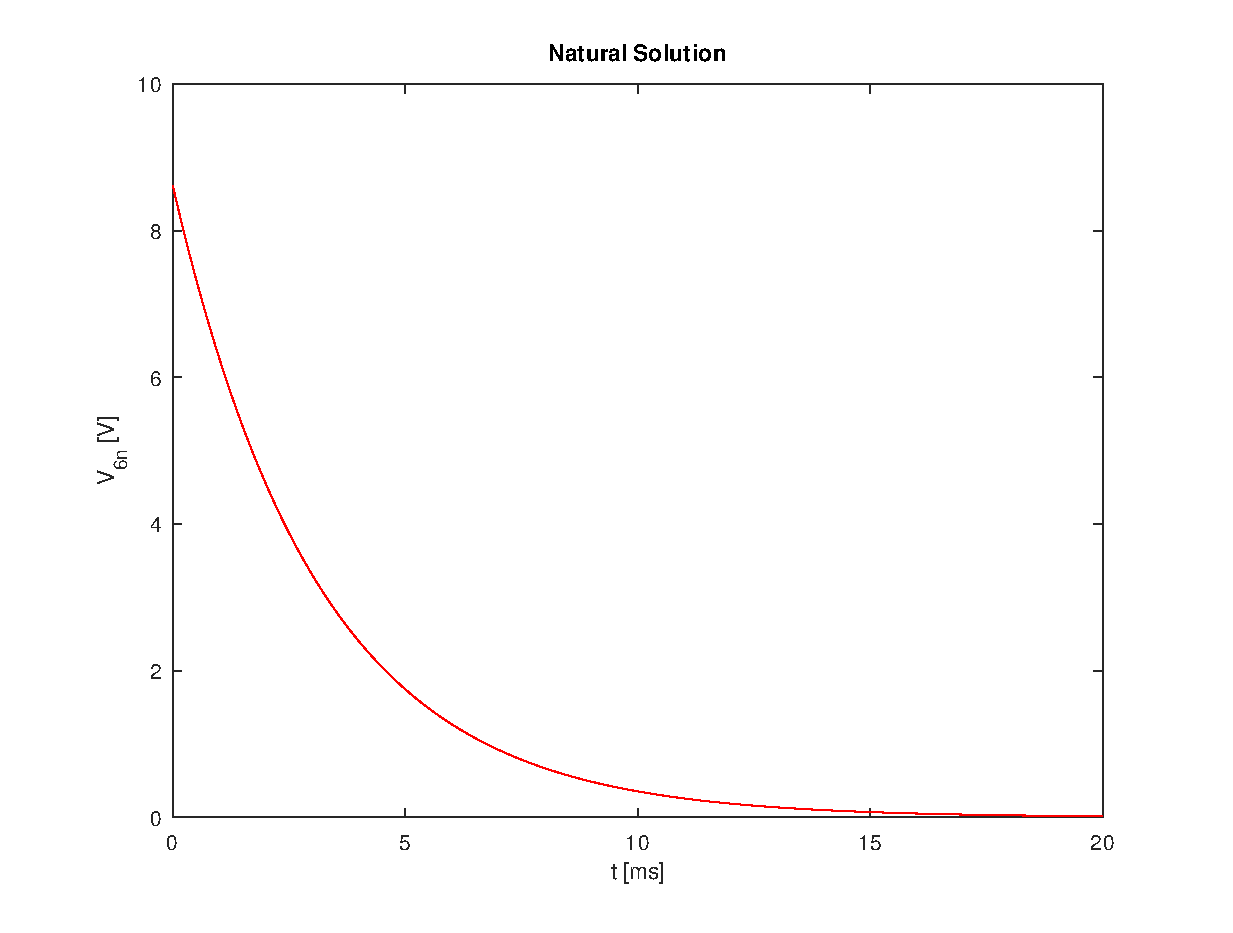
\includegraphics[width=0.8\linewidth]{nat_sol.eps}
  \caption{Natural Solution - $v_6$}
  \label{fig:natural solution}
\end{figure}


\newpage
\subsection{Forced Solution}
\label{subsec:forced_solution}

In this section we obtain the forced solution, $v_{6f}$, for $f=1kHz$.
To achieve the wanted result we use a phasor voltage source, $v_{s}=1$, wich as the complex value of $\bar{v_{s}}=e^{(-(\pi/2)*j)}$.
It is also needed to replace the capacitor, $C$ with its impedance, $Z_C$, wich is given by: $Z_{C}= 1/(j*\omega*C)$, where $\omega=2*\pi*f$ is the angular frequency.
In order to facilitate writing the equations we use $G_C$ as $\frac{1}{Z_C}$.
This procedure allow us to solve the circuit using the Node Method, by solving the following system

$$
\begin{bmatrix}
  1 & 0 & 0 & 0 & 0 & 0 & 0 \\
  G_{1} & -G_{1}-G_{2}-G_{3} & G_{2} & G_{3} & 0 & 0 & 0 \\
  0 & G_{2}+K_{b} & -G_{2} & -K_{b} & 0 & 0 & 0 \\
  0 & G_{3} & 0 & -G_{3}-G_{4}-G_{5} & G_{5}+G_{C} & G_{7} & -G_{C} -G_{7} \\
  0 & -K_{b} & 0 & K_{b}+G_{5} & -G_{5}-G_{C} & 0 & G_{C} \\
  0 & 0 & 0 & 0 & 0 & -G_{6}-G_{7} & G_{7} \\
  0 & 0 & 0 & 1 & 0 & K_{d}*G_{6} & -1
\end{bmatrix}
=
\begin{bmatrix}
  V_{1}\\
  V_{2}\\
  V_{3}\\
  V_{5}\\
  V_{6}\\
  V_{7}\\
  V_{8}
\end{bmatrix}
\begin{bmatrix}
  V_{s}\\
  0\\
  0\\
  0\\
  0\\
  0\\
  0
\end{bmatrix}
$$

that give us the complex amplitudes in each node:
\begin{table} [H]
  \centering
  \begin{tabular}{|l|r|}
    \hline    
    {\bf Name} & {\bf Value [V]} \\ \hline
    $V_1$ & $1.000000e^{-1.570796j}$ \\ \hline 
$V_2$ & $0.956740e^{-1.570796j}$ \\ \hline 
$V_3$ & $0.867448e^{-1.570796j}$ \\ \hline 
$V_4$ & $0.000000e^{0.000000j}$ \\ \hline 
$V_5$ & $0.962802e^{-1.570796j}$ \\ \hline 
$V_6$ & $0.583850e^{1.717262j}$ \\ \hline 
$V_7$ & $0.385459e^{1.570796j}$ \\ \hline 
$V_8$ & $0.581928e^{1.570796j}$ \\ \hline 

  \end{tabular}
  \caption{Complex Amplitudes in each node}
  \label{tab:volt3}
\end{table}


\newpage
\subsection{Total Solution}
\label{subsec:total_solution}

Finally, in order to obtain the total solution we set $v_{s}=sin(w*t)$ and solve the linear differencial equation \ref{eq:kvl2} whose solution is a superposition of the natural solution $v_{6n}$ and the forced solution $v_{6f}$:

\begin{equation}
  v_6(t) = v_{6n}(t) + v_{6f}(t).
  \label{eq:v6_sol}
\end{equation}

The outcome is displayed in the next plot:

\begin{figure}[H] \centering
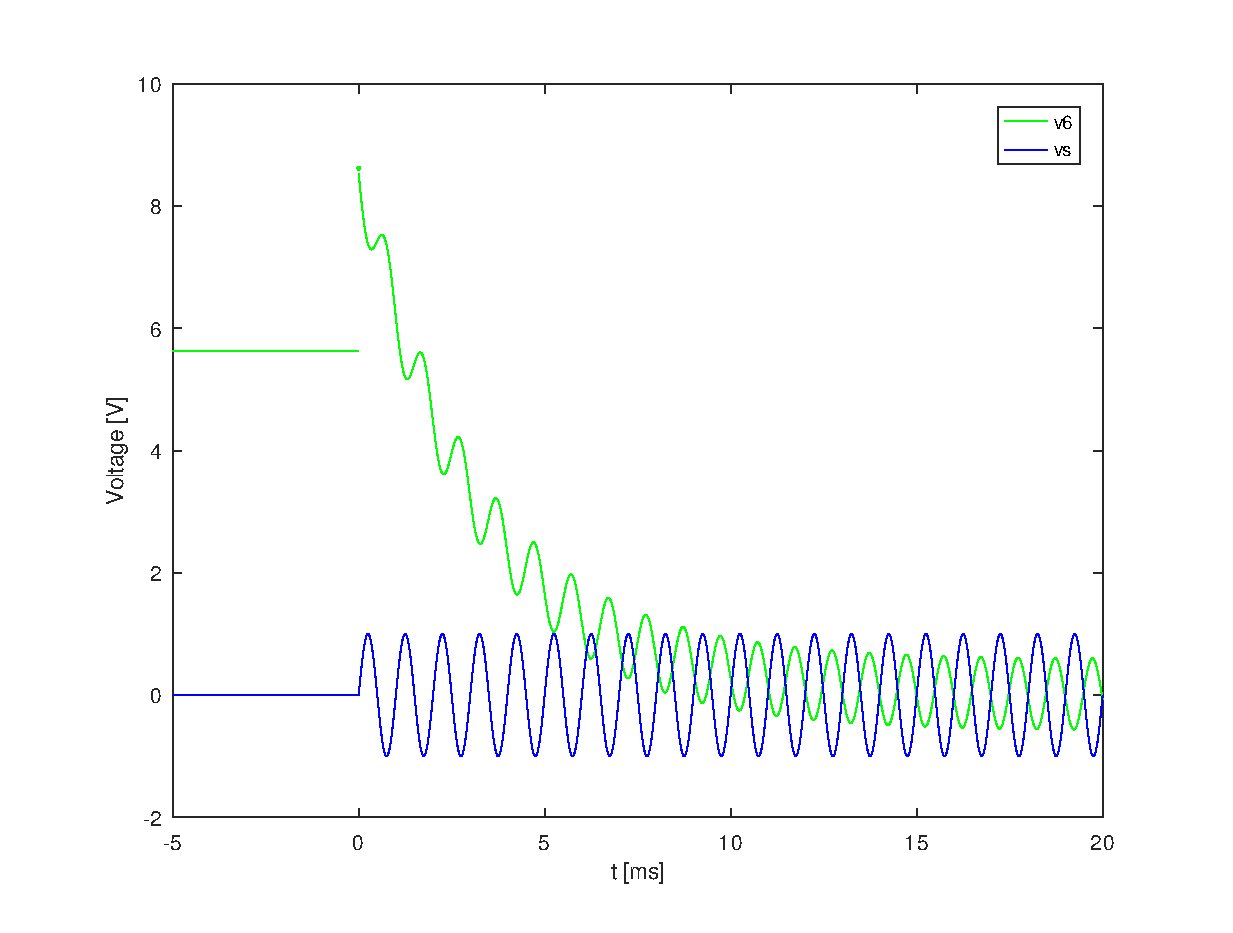
\includegraphics[width=0.8\linewidth]{tot_sol.eps}
\caption{Total solution - $v_6$}
\label{fig:total solution}
\end{figure}


\newpage
\subsection{Frequency Response}
\label{subsec:frequency_response}

To finish the analysis on this circuit we study its frequency response for frequency range 0.1Hz to 1MHz. To do that we represent bellow the plots of both the magnitude and the phase of $V_{c}(f)=V_{6}(f)-V_{8}(f)$, $V_{s}(f)$ and $V_{6}(f)$.
To find this quantities we just solve the system presented in Section \ref{subsec:forced_solution} in loop, determining the transfer functions for each of the frequency values.
\par The tranfer function of each quantity is given by:
$$
\begin{cases}
  H_{6}=\frac{\bar{v_{6}}}{\bar{v_{s}}}\\
  H_{C}=\frac{(\bar{v_{6}}-\bar{v_{8}})}{\bar{v_{s}}}\\
  H_{s}=\frac{\bar{v_{s}}}{\bar{v_{s}}}
\end{cases}
$$


To do the plot we need to create a logharitmicaly spaced vector of frequencies. In doing so we end up with a vector of magnitudes and a vector of phases for each of the node voltages. With this procedure coming up with the plots consists on ploting each one of the vector's magnitude and phase against frequency.

So the magnitude is obtained by:
$$
\begin{cases}
  \text{Magnitude}\: \bar{v_{6}} = abs(H_{6})\\
  \text{Magnitude}\: \bar{v_{C}} = abs(H_{C})\\
  \text{Magnitude}\: \bar{v_{s}} = abs(H_{s})  
\end{cases}
$$
\begin{figure}[H] \centering
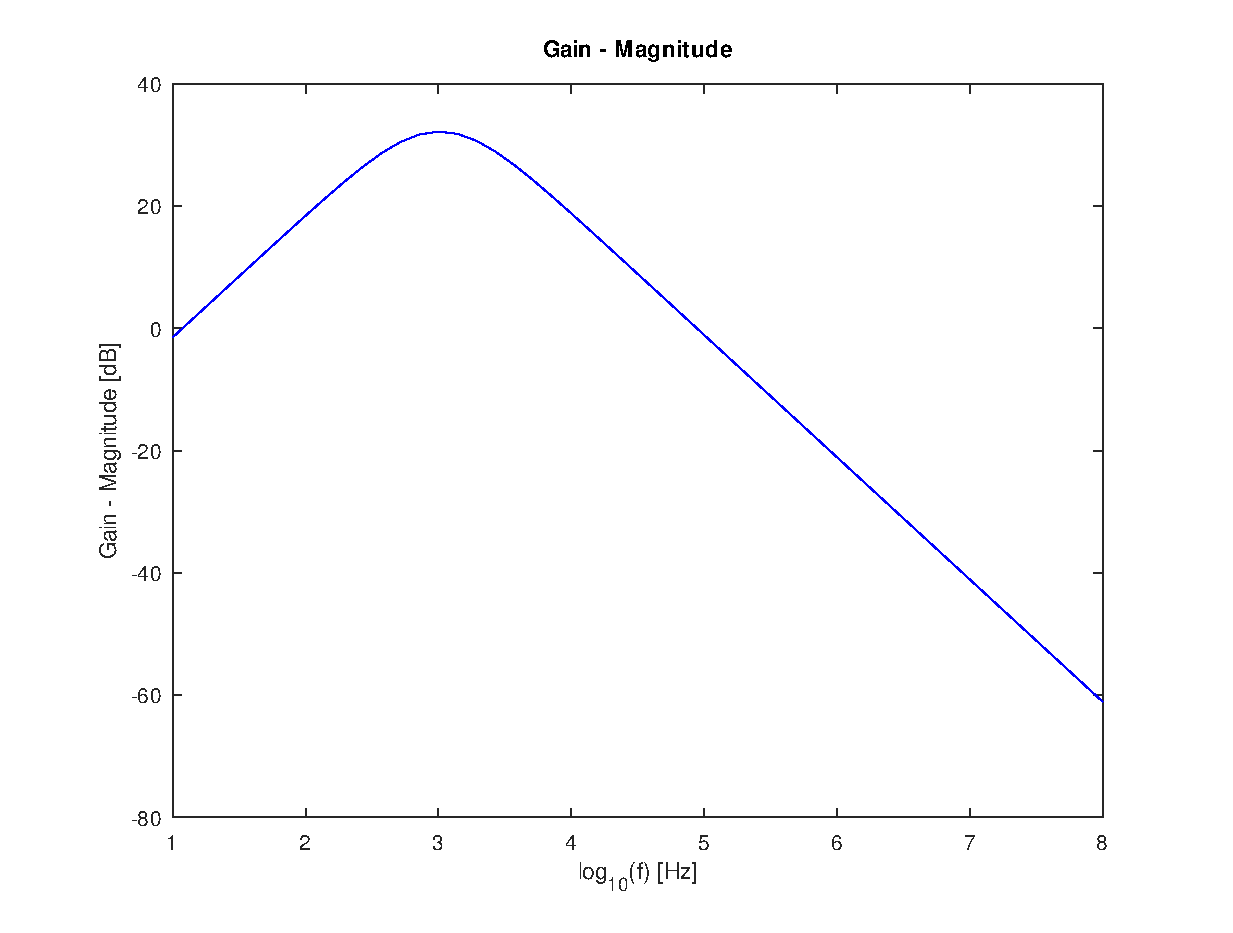
\includegraphics[width=0.8\linewidth]{freq_db.eps}
\caption{Magnitude of the frequency response of $v_s(f)$, $v_c(f)$ and $v_6(f)$}
\label{fig:magnitude_theo}
\end{figure}

Analysing the plot above one understands easely why $\bar{v_s}$'s magnitude is zero. Its magnitude is 1, but since the plots are represented on a logarithmic scale is value in that scale is 0.
Looking for $\bar{v_C}$'s magnitude one realizes that the highest the frequency the lowest the magnitude. When the frequency tends to infinity, it eventualy tends to zero, because the capacitor can not keep up its charging an discharging rithym with the rate of frequency oscilation.
%FALTA O V6!?!?!?

Phase can be computed from the formulas bellow:
$$
\begin{cases}
  \text{Phase}\: \bar{v_{6}} = angle(H_{6})\\
  \text{Phase}\: \bar{v_{C}} = angle(H_{C})\\
  \text{Phase}\: \bar{v_{s}} = angle(H_{s})
\end{cases}
$$

\begin{figure}[H] \centering
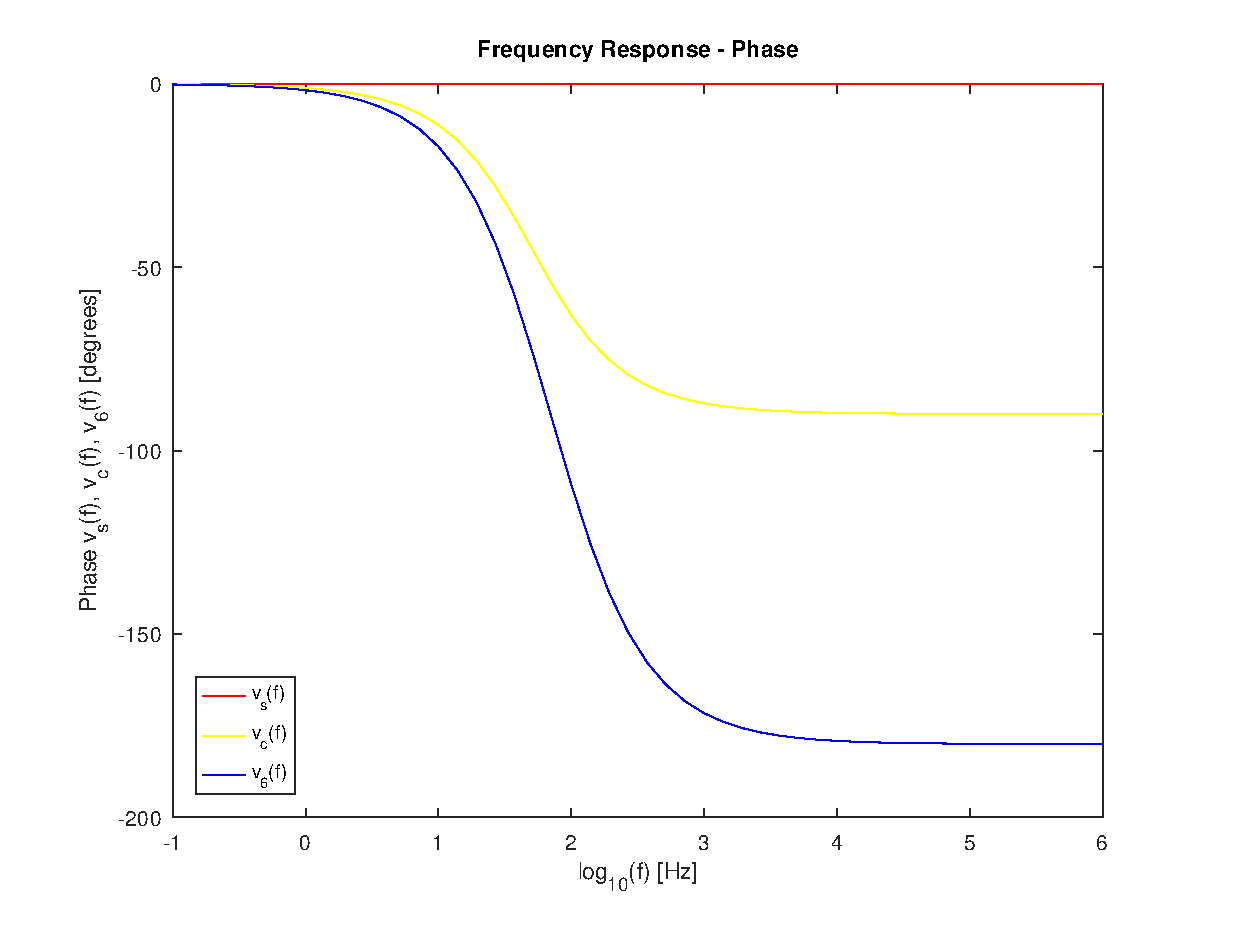
\includegraphics[width=0.8\linewidth]{phase_ang.eps}
\caption{Magnitude of the frequency response of $v_s(f)$, $v_c(f)$ and $v_6(f)$}
\label{fig:phase_theo}
\end{figure}

From this plot one observes that the phase of  $\bar{v_s}$ is constant and equal to zero since it is the input source, and therefore, all other phases depend on its.
The capacitor's phase it's initialy zero degrees and tends to -90 degrees as the frequency tends to infinity. This is justified by the value of its impedance wich as a phase of exactly -90 degrees. The phase varies continuously since the capacitor tries to keep up with the variation of $\omega$. Notice that the voltages in the circuit have diferent phases because this is not a linear circuit, because it contains one capacitor. If the circuit only had resistors, the phases would be the same.
%FALTA V6 !?!?!?!?!'

